\documentclass[12pt,reqno]{article}
\usepackage{amsmath}

\usepackage[text={180mm,250mm},centering]{geometry}                % See geometry.pdf to learn the layout options. There are lots.
\geometry{a4paper}                   % ... or a4paper or a5paper or ...

%\geometry{landscape}                % Activate for for rotated page geometry
%\usepackage[parfill]{parskip}    % Activate to begin paragraphs with an empty line rather than an indent

\usepackage{graphicx}
\usepackage{amssymb}
\usepackage{epstopdf}
\usepackage{enumerate}

\usepackage{amsmath,amsthm}
\usepackage{tikz}


\usepackage[mathscr]{eucal}
\usepackage[all]{xy}
\usepackage{mathrsfs}
\usepackage{authblk}
\usepackage{hyperref}
\usepackage{natbib}

%\usepackage{times}
%\usepackage{times}\usepackage{mathptmx}
%\usepackage{charter}

%\usepackage{fourier}
%\usepackage{times}\usepackage[mtbold,mtpluscal,mtplusscr]{mathtime}

\usepackage{titlesec}

\titleformat{\section}{\Large}{Lecture\, \thesection}{1em}{}

\linespread{1.2}

\newcommand{\N}{\mathbb{N}}
\newcommand{\R}{\mathbb{R}}
\newcommand{\Q}{\mathbb{Q}}
\newcommand{\Z}{\mathbb{Z}}
\newcommand{\CC}{\mathbb{C}}

\newcommand{\OO}{\mathcal{O}}
\newcommand{\B}{\mathcal{B}}
\newcommand{\cU}{\mathcal{U}}

\newcommand{\rO}{\mathrm{O}}

\newcommand{\op}{\mathrm{op}}
\newcommand{\rd}{\mathrm{d}} %roman d
\newcommand{\GL}{\mathrm{GL}}
\newcommand{\SU}{\mathrm{SU}}
\newcommand{\SL}{\mathrm{SL}}
\newcommand{\SO}{\mathrm{SO}}
\newcommand{\U}{\mathrm{U}}
\newcommand{\Sp}{\mathrm{Sp}}




\theoremstyle{definition}
\newtheorem{theorem}{Theorem}[section]
\newtheorem{lemma}[theorem]{Lemma}
\newtheorem{conjecture}[theorem]{Conjecture}
\newtheorem{corollary}[theorem]{Corollary}

\newtheorem{claim}[theorem]{Claim}
\newtheorem{fact}[theorem]{Fact}
\newtheorem{question}[theorem]{Question}




\newtheorem{prop}[theorem]{Proposition}
\newtheorem{example}[theorem]{Example}
\newtheorem{definition}[theorem]{Definition}
\newtheorem{definition-lemma}[theorem]{Definition-Lemma}
\newtheorem{definition-theorem}[theorem]{Definition-Theorem}

\newtheorem{proposition-example}[theorem]{Proposition-Example}

\newtheorem{remark}[theorem]{Remark}
\newtheorem*{remarks}{Remarks}

\newtheorem*{ack}{Acknowledgements}
\newtheorem*{convention}{Convention}


%\newcommand{\ac}{\textup{!`}}


%\def\ldb{\mathopen{\{\!\!\{}}
%\def\rdb{\mathclose{\}\!\!\}}}
%\def\ldbg{\mathopen{\bigl\{\!\!\bigl\{}}
%\def\rdbg{\mathclose{\bigr\}\!\!\bigr\}}}
%\def\ldbgg{\mathopen{\Bigl\{\!\!\Bigl\{}}
%\def\rdbgg{\mathclose{\Bigr\}\!\!\Bigr\}}}

\allowdisplaybreaks



%============================================================



\title{Complex Analysis I}
\author{Matthias Weber\\
 {\small Indiana University, Bloomington}}

\renewcommand\Affilfont{\small}

\affil{Notes taken by Aolong Li}
\date{}



\begin{document}

\maketitle

 Complex analysis interacts in many ways with ordinary and partial differential equations
(harmonic functions), geometry (conformal mapping), number theory, algebraic
geometry, and everything else. It opens the doors to riemann surfaces, complex dynamics,
and several complex variables\\ \vspace{3pt}
  
\begin{figure}[h!]
\centering
\includegraphics[width=0.8\textwidth]{Mandel.eps}
\footnotemark
\end{figure}
\footnotetext{Mandelbrot set. Initial image of a zoom sequence: Mandelbrot set with continuously colored environment. Coordinates of the center: $\mathrm{Re}(c) = -.7, \ ~ \mathrm{Im}(c) = 0$;
Horizontal diameter of the image: $3.076,9$; Created by Wolfgang Beyer with the program Ultra Fractal $3$. From \href{https://commons.wikimedia.org/wiki/File:Mandel_zoom_00_mandelbrot_set.jpg}{Wikipedia.org}.}


\newpage
 This course will be mostly based on {\it Complex Analysis } (Eberhard Freitag and Rolf Busam)
and {\it Complex Analysis II} (Eberhard Freitag), but also hand out a class diary with complete
proofs.

\tableofcontents

\newpage

\section{August 22, 2017}
\subsection{Introduction}
We are going to discuss the classical theory of holomorphic functions in the complex plane:
\begin{itemize}
    \item Holomorphic Functions
    \item Cauchy’s Integral Theorem
    \item Meromorphic Functions and Residue Theorem
    \item Power Series, Products, Partial Fractions
    \item Riemann Mapping Theorem
    \item Harmonic Functions
    \item Elliptic Functions
\end{itemize}
 
 
\subsection{Complex Numbers}
A complex number is $z=a+b\sqrt{-1}$ where $a,b\in \R$. Also, we can write $z=(a,b)$. Especially, we can write $\sqrt{-1}=i=(0,1)$. The main difference between $\CC$ and $\R^2$ is the multiplication:
\[z\cdot z'=(aa'-bb',ab'+a'b) \]

Note that $\CC$ cannot be an ordered field.\footnote{A field $(F,+, \times)$ together with a total order $\leq$ on $F$ is an ordered field if the order satisfies the following properties for all $a, b$ and $c$ in $F$: (1) if $a \leq b$ then $a + c \leq b + c$; and (2)
if $0 \leq a$ and $0 \leq b$ then $0 \leq a \times b$.} \\

Define the norm of $z$ as $|z|^2=z\bar{z}$. It can be verified that 
\[|z\cdot w|=|z|\cdot|w|\]
We can check this directly, or treat complex numbers as matrices and the multiplication as the multiplication of matrices:
\[z=\begin{pmatrix}a&b\\-b&a\end{pmatrix},\quad w=\begin{pmatrix}c&d\\-d&c\end{pmatrix}\quad a,b,c,d\in \R\]
and 
\[zw=\begin{pmatrix}a&b\\-b&a\end{pmatrix}\begin{pmatrix}c&d\\-d&c\end{pmatrix}=\begin{pmatrix}ac-bd&ad+bc\\-(ad+bc)&ac-bd\end{pmatrix}.\]
Hence the ``rules of norm'' can be obtained immediately by
\[\det (AB)=\det A \det B.\]

An interesting interpretation is the product of two square sums can be written as a sum of two square numbers, since 
\[|a+bi|^2=a^2+b^2\]
For example,
\[1^2+2^2=5,\quad 2^2+3^2=13 \]
and 
\[5\times 13=65=4^2+7^2\]

\subsection{Holomorphic Functions}
\begin{definition}
Let $f$ be defined and complex valued in an open neighborhood of a point $z_0$. Then $f$ is holomorphic (or analytic, or complex differentiable) at $z_0$ if 
\[\lim_{z\to z_0}\frac{f(z)-f(z_0)}{z-z_0}\]
exists.\par
$f$ is holomorphic in an open set $U$ if it is holomorphic at every point of $U$. The set of all such $f$ is denoted by $\OO(U)$.
\end{definition}

\begin{example}
As in real analysis, 
\begin{enumerate}
\item $f(z)\equiv \text{constant}$ $\Rightarrow$ $f'(z)=0$;
\item $f(z)=z$ $\Rightarrow$ $f'(z)=1$;
\item For $f,g\in \OO(U)$, we have
\[(f+g)'=f'+g',\quad (fg)'=f'g+fg',\quad \left(\frac{f}{g}\right)'=\frac{gf'-g'f}{g^2}\]
\item Polynomials are holomorphic, rational functions are holomorphic.
\end{enumerate}
\end{example}

\begin{theorem}
Let $c_1(t)$ and $c_2(t)$ be differentiable curves in an open set $U$, and let $f\in \OO(U)$, then we have
\[\frac{\rd}{\rd t}f(c(t))=f'(c(t))\cdot c'(t).\]
\end{theorem}
\begin{remark}
The multiplication on the right side is the multiplication of complex numbers.
\end{remark}
\begin{proof}
Assume $c'(t_0)\neq 0$. Consider
\[\begin{aligned}\lim_{t\to t_0} \frac{f(c(t_0)-f(c(t)))}{t_0-t}&=\lim_{t\to t_0} \frac{f(c(t_0)-f(c(t)))}{c(t_0)-c(t)}\cdot\frac{c(t_0)-c(t)}{t_0-t}\\
&=f'(c(t_0))\cdot c'(t_0)\end{aligned}.\]
Now assume $c'(t_0)=0$. We need to show
\[\lim_{t\to t_0} \frac{f(c(t_0)-f(c(t)))}{t_0-t}=0.\]
Let $w_0=c(t_0)$, then 
\[\left|\frac{f(w_0)-f(w)}{w_0-w}\right|\leq C \quad \text{for $w$ near $w_0$ ,}\]
i.e.
\[\left|f(w_0)-f(w)\right|\leq C \cdot\left|w_0-w\right|.\]
Then we have 
\[\left|\frac{f(c(t_0))-f(c(t))}{t_0-t}\right|\leq C\left|\frac{c(t_0)-c(t)}{t_0-t}\right|\xrightarrow{\ ~t\to t_0~\ } 0\]
\end{proof}
\begin{corollary}
$f$ preserves the angle between the tangent vectors of two intersecting curves at the intersect point.
\end{corollary}

\subsection{M\"obius Transformations}
Consider the {\it M\"obius transformation}:
\[f(z)=\frac{az+b}{cz+d}\]
And we can rewrite this:
\[\begin{aligned}f(z)&=\dfrac{\dfrac{a}{c}(cz+d)+b-\dfrac{ad}{c}}{cz+d}\\
   &=\dfrac{a}{c}+\left(b-\dfrac{ad}{c}\right)\dfrac{1}{cz+d}\end{aligned}\]
 Then the M\"obius transformation is decomposed into three kinds of transformation: transition, scalar multiplication and reciprocity. Thus, we can focus on these three simple transformations:
 \begin{enumerate}
 \item $f(z)=a\cdot z$: scalar if $a\in \R$; rotates if $a=e^{it}=\cos t+i\sin t$, and for every $a\in \CC$, it can be written as $a=|a|\cdot e^{i~\mathrm{arg}~a}$, so this case is clear;
 \item $f(z)=z+c$ for some constant $c\in \CC$: simple;
 \item $f(z)=\frac{1}{z}$ is related to $I(z)=\frac{z}{|z|^2}$, since 
 \[I(z)=\frac{1}{\bar{z}}\quad \Rightarrow \quad I(\bar{z})=\frac{1}{z} \]
 For $I(z)$, we have the following results:
 \begin{theorem}
 The map $I:\CC\rightarrow \CC$ sending 
 \begin{itemize}
 \item lines through $0$ to lines through $0$;
 \item lines through $0$ to circles through $0$;
 \item circles not through $0$ to circles not through $0$;
 \end{itemize}
 {\it vice versa}, since $I^2=\mathrm{id}$.\end{theorem}
  \end{enumerate}

 
\begin{figure}
\centering
\begin{minipage}{.3\textwidth}
  \centering
  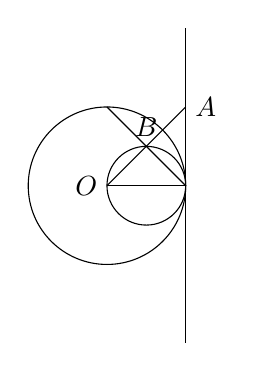
\begin{tikzpicture}
          \draw (1,2)--(1,-2);
          
          \draw (0.5,0) circle [radius=0.5];
          \draw (0,0) circle [radius=1];
          \draw (0,0) node[left]{$O$}--(1,1) node[right]{$A$};
          \draw (1,0)--(0,1);
          \draw (0,0)--(1,0);
          \node[above] at (0.5,0.5) {$B$};
          \end{tikzpicture} 
\caption{Case A}
\end{minipage}%
\begin{minipage}{.3\textwidth}
  \centering
   \begin{tikzpicture}
          \draw (2,2)--(2,-2);
          \draw (1,2)--(1,-2);
          \draw (0.3,0) circle [radius=0.3];
          \draw (0,0) circle [radius=1];
          \end{tikzpicture}
  \caption{Case B}
\end{minipage}%
\begin{minipage}{.3\textwidth}
  \centering
    \begin{tikzpicture}
          \draw (1,2)--(1,-2);
          \draw (2,0) circle [radius=1];
          \draw (0,0) circle [radius=1];
          \end{tikzpicture}
  \caption{Case C}
\end{minipage}
\end{figure}

 Let us look at several special cases:
 
\begin{itemize}
     \item $\dfrac{1}{z}$ maps the line tangent to unit circle to a circle through $O$. In fact, by Thales' theorem, we know there are two right angles. It follows that $|OA|\cdot |OB|=1$.
     \item $\dfrac{1}{z}$ maps the vertical line (not through $O$) to a circle through $O$. Indeed, suppose $R(z)=r\cdot z$, $(r>0)$, we have $I=RIR$. Namely,
     \[R(I(R(z)))=R(I(rz))=r\frac{rz}{|rz|^2}=\frac{z}{|z|^2}=I(z).\]
     So, equivalently, we can maps a vertical line to another vertical line tangent to the circle, then maps the new line to a circle. Finally, we maps to the circle to another circle. Hence we maps the vertical line to a circle eventually.
     \item $\dfrac{1}{z}$ maps a circle $C$ touching unit circle at $1$ to a circle. Consider 
     \[\frac{1}{z-1}\]
     maps $C$ to a vertical line (transition+reciprocity). Then
     \[\dfrac{1}{1+\dfrac{1}{z-1}}\]
     maps $C$ to a circle. And 
     \[\frac{1}{z}=1-\dfrac{1}{1-\dfrac{1}{1-z}}\]
     Hence $\dfrac{1}{z}$ maps a circle $C$ touching unit circle at $1$ to a circle eventually.
 \end{itemize}
 
 \begin{remark}
 We have the equality:
 \[\dfrac{1}{1+\dfrac{1}{z-1}}=1-\dfrac{1}{z},\]
 equivalently,
 \[\dfrac{1}{z}=1-\dfrac{1}{1-\dfrac{1}{1-z}}.\]
 Therefore, we have 
 \[z=\dfrac{1}{1-\dfrac{1}{1-\dfrac{1}{1-z}}}\]
 There is another viewpoint to say why the above equation holds. We have the theorem:
 \begin{theorem}
 For any three distinct ponits $a,b,c\in\CC$, there is a unique M\"obius transformation $\mu(z)$ with 
 \[\mu(a)=0,\quad \mu(b)=\infty,\quad \mu(c)=1.\]
 \end{theorem}
 \begin{proof}
 To meet the requirement, we have the following attempts step by step:
 \[\frac{\lambda(z-a)}{\cdots}~\rightarrow~ \frac{\lambda(z-a)}{\lambda' (z-b)}~\rightarrow~ \lambda\cdot\frac{z-a}{z-b}~\rightarrow~ \frac{c-b}{c-a}\cdot\frac{z-a}{z-b}:=\mu(z)\]
 \end{proof}
 Let $\mu(z)=\dfrac{1}{1-z}$, then 
 \[\mu(\mu(\mu(z)))=\dfrac{1}{1-\dfrac{1}{1-\dfrac{1}{1-z}}}\]
 and note that 
 \[\mu(0)=1,\quad \mu(1)=\infty,\quad \mu(\infty)=0,\]
 and 
 \[\mu^3(0)=0,\quad \mu^3(1)=1,\quad \mu^3(\infty)=\infty.\]
 Hence $\mu^{3}=\mathrm{id}$.

 \end{remark}
   
\newpage 
\bibliographystyle{plain}
\bibliography{references}
\end{document}
